\documentclass{article}

\usepackage{graphicx}
\usepackage{tikz}
\usepackage{tikzsymbols}
\usetikzlibrary{calc,patterns,shapes.geometric}
\pagestyle{empty}
\usepackage[margin=0pt]{geometry}
\geometry{papersize={14in,12in}}

\def\centerarc[#1](#2)(#3:#4:#5){\draw[#1] ($(#2)+({#5*cos(#3)},{#5*sin(#3)})$) arc (#3:#4:#5);}

\begin{document}
	\begin{figure}
		\centering
		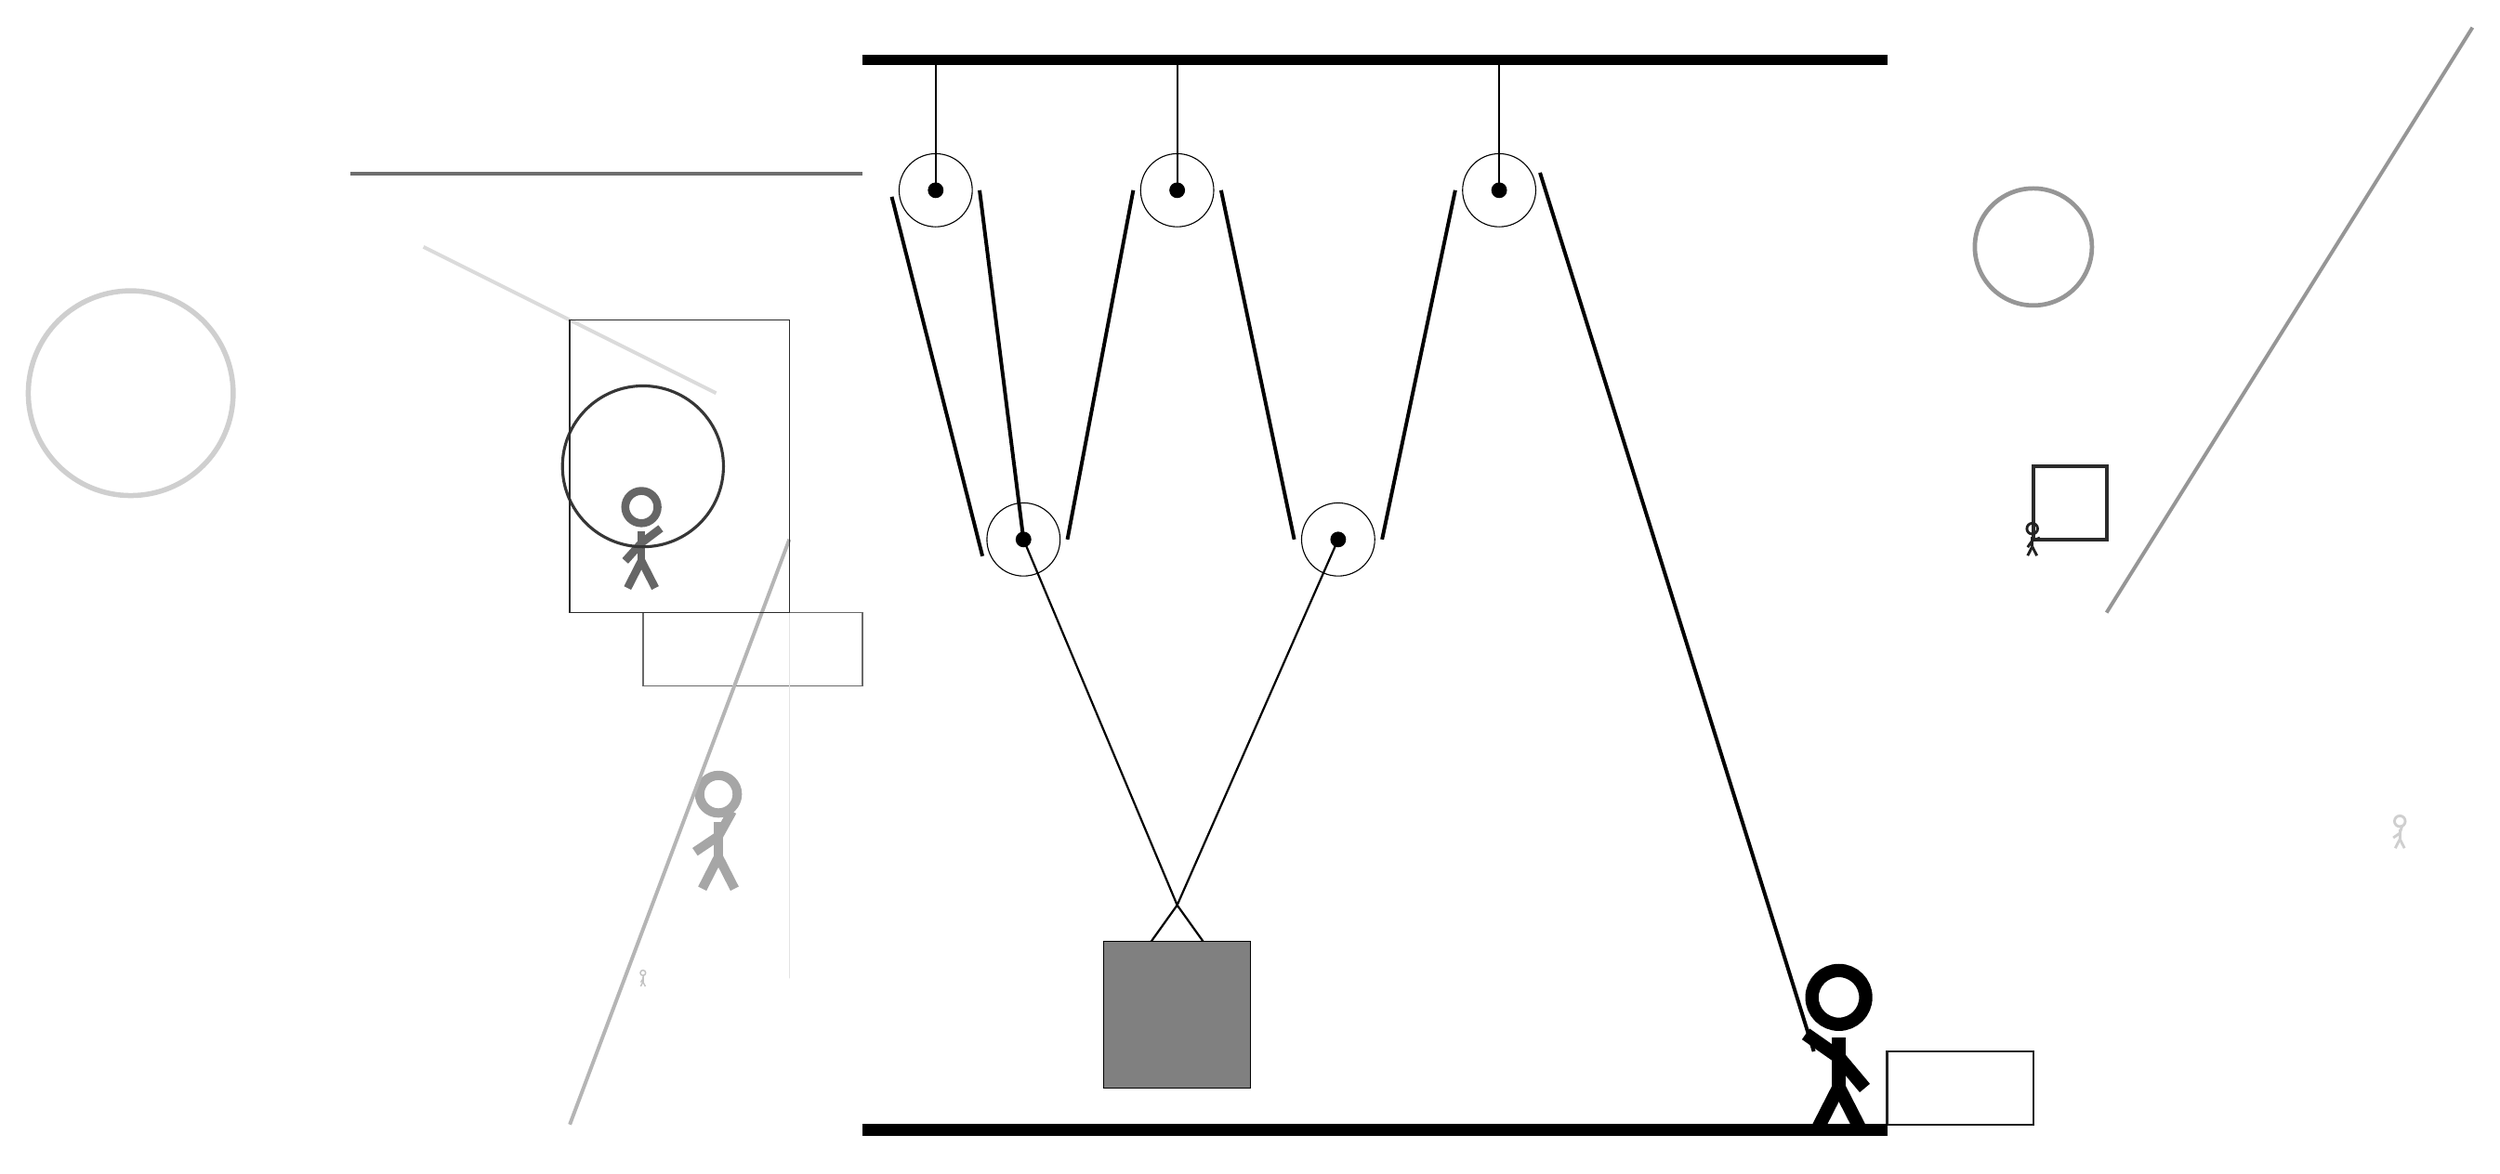
\begin{tikzpicture}
			%%%%% START %%%%%
			
			\draw[fill=black] (-2, 11.5) rectangle (12, 11.625);
			
			\draw (-1, 9.775) circle (0.5);
			\draw[fill=black] (-1, 9.775) circle (0.1);
			\draw[thick] (-1, 9.775) -- (-1, 11.5);
			
			\draw (2.3, 9.775) circle (0.5);
			\draw[fill=black] (2.3, 9.775) circle (0.1);
			\draw[thick] (2.3, 9.775) -- (2.3, 11.5);
			
			\draw (6.7, 9.775) circle (0.5);
			\draw[fill=black] (6.7, 9.775) circle (0.1);
			\draw[thick] (6.7, 9.775) -- (6.7, 11.5);
			
			\draw (0.2, 5) circle (0.5);
			\draw[fill=black] (0.2, 5) circle (0.1);
			
			\draw (4.5, 5) circle (0.5);
			\draw[fill=black] (4.5, 5) circle (0.1);
			
			\draw[line width=0.5mm, color=black!57](-2, 10) -- (-9, 10);
			
			\node[line width=0.3mm, color=black!24] at (-5, -1) {\Strichmaxerl[1][58][81]};
			\node[line width=0.5mm, color=black!35] at (-4, 1) {\Strichmaxerl[7][34][61]};
			\draw [line width=0.7mm, color=black!19](-12, 7) circle (1.4);
			
			\draw[line width=0.2mm, color=black!59] (-2, 3) rectangle (-5, 4);
			\draw [line width=0.6mm, color=black!41](14, 9) circle (0.8);
			\draw[line width=0.5mm, color=black!83] (14, 6) rectangle (15, 5);
			\node[line width=0.5mm, color=black!87] at (14, 5) {\Strichmaxerl[2][55][20]};
			\draw[line width=0.2mm, color=black!11] (-3, 6) rectangle (-3, -1);
			\draw[line width=0.5mm, color=black!14](-4, 7) -- (-8, 9);
			
			\node[line width=0.7mm, color=black!60] at (-5, 5) {\Strichmaxerl[6][48][37]};
			\node[line width=0.6mm, color=black!19] at (19, 1) {\Strichmaxerl[2][35][73]};
			\draw[line width=0.5mm, color=black!29](-3, 5) -- (-6, -3);
			
			\draw[line width=0.3mm, color=black!87] (14, -2) rectangle (12, -3);
			\draw [line width=0.4mm, color=black!79](-5, 6) circle (1.1);
			\draw[line width=0.2mm, color=black!83] (-3, 4) rectangle (-6, 8);
			
			\draw[line width=0.5mm, color=black!41](15, 4) -- (20, 12);
			
			\draw[thick] (0.2, 5) -- (2.3, 0)  -- (4.5, 5);
			\draw[thick]  (1.8, -0.7) -- (2.3, 0) -- (2.8, -0.7);
			\draw[fill=black!50] (1.3, -0.5) rectangle (3.3, -2.5);
			
			\draw[line width=0.5mm] (0.2, 5) -- (-0.4, 9.775);
			\centerarc[line width=0.5mm](-1, 9.775)(0:200:0.6);
			\draw[line width=0.5mm] (-1.6, 9.685) -- (-0.361, 4.772);
			\centerarc[line width=0.5mm](0.2, 5)(200:360:0.6);
			\draw[line width=0.5mm](0.8, 5) -- (1.7, 9.775);
			\centerarc[line width=0.5mm](2.3, 9.775)(0:180:0.6);
			\draw[line width=0.5mm] (2.9, 9.775) -- (3.9, 5);
			\centerarc[line width=0.5mm](4.5, 5)(180:360:0.6);
			\draw[line width=0.5mm] (5.1, 5) -- (6.1, 9.775);
			\centerarc[line width=0.5mm](6.7, 9.775)(20:180:0.6);
			\draw[line width=0.5mm](7.258, 10.015)  -- (11, -2);
			
			\node at (11.3, -2) {\Strichmaxerl[10][-35][-50]};
			
			\draw[fill=black] (-2, -3) rectangle (12, -3.15);
			
			%%%%% END %%%%%
		\end{tikzpicture}
	\end{figure}	
\end{document}